\documentclass{article}[14pt]

\usepackage{amsmath}
\usepackage{amssymb}
\usepackage{graphicx}
\usepackage{float}
\usepackage{array}
\usepackage{tikz}
\usepackage{latexsym}
\usepackage{xspace}
\usepackage{algpseudocode}
\usepackage{algorithm}
\usepackage{verbatim}

\setlength{\textheight}{9in}
\setlength{\textwidth}{6.5in}
\setlength{\columnsep}{0.3125in}
\setlength{\topmargin}{-0in}
\setlength{\headheight}{-0in}
\setlength{\headsep}{0in}
\setlength{\parindent}{1pc}
\setlength{\oddsidemargin}{0in}

%\parindent=0pt

\title{Robust Non-linear MPC (NL-RMPC) via Feedback Linearization}
\author{YVP, HA. JD, RM}

\begin{document}
\maketitle

\section{Quick intro to feedback linearization for MIMO Systems}

Consider the control affine non-linear dynamics:
\begin{subequations}
\begin{align}
\dot{x}&=f(x)+G(x)u \\
y&=h(x)
\end{align}
\end{subequations}
Where $x\in\mathbb{R}^n$, $u\in\mathbb{R}^m$ and $y\in\mathbb{R}^m$.

\textbf{[Assumption]:} Without loss of generality, assume that the system has a vector relative degree (\textbf{[L8,Def2.1]}) $\rho_1,\dotsc,\rho_m$ s.t. $\sum_{i=0}^m \rho_i=n$ in a region of the state space $D\in\mathbb{R}^n$. Consequently, the system also satisfies \textbf{[L8,Th2.8]} and \textbf{[L8,Prop2.7]}. From \textbf{[L8,Def2.1]}, there exists a matrix $A(x)$, which is full rank $\forall x \in D$. Also, there exists a vector $b(x) \in \mathbb{R}^n$ as defined in \textbf{[L8]}. Under these assumptions, a control law of the form

\begin{subequations}
\begin{align}
u&=A(x)^{-1}(-b(x)+v) \\
&=-A(x)^{-1}b(x)+A(x)^{-1}v
\end{align}
\end{subequations}

And a state transformation (which is a diffeomorphism in $D$) of $z=T(x)$ (as defined in \textbf{[L8,Th2.4]}, the non-linear system can be written in the form:

\begin{subequations}
\begin{align}
\dot{z}&=Az+Bv 
%\text{Where, } \nonumber \\
%A&=\begin{bmatrix} 0 & 1 & 0 & \dotsc \\ 0 & 0 & 1 & \dotsc \\ {}& {}& \ddots &{}\\ {}& \dotsc & {} & 0  \end{bmatrix}
\end{align}
\end{subequations}

\section{Problem formulation}
The control problem is as follows:

\begin{subequations}
\begin{align}
\text{Minimize } &l(x,u) \\
&\text{s.t.} \nonumber \\
\dot{x}&=f(x)+G(x)u \\
x&\in X\\
u&\in U
\end{align}
\end{subequations}

A state-estimator provides (potentially delayed) access to a state estimate \begin{subequations}
\begin{align}
\hat{x}(t)&=x(t)+e(t) \\ 
\text{where, } e(t) &\in E
\end{align}
\end{subequations}

The control problem now becomes one of robust control of the system in order to minimize a control cost while guaranteeing safety of the system ($x\in X$) and respecting the limits on the control input ($u \in U$) with access to the state-estimate with error as described above. 

Note, we assume $X$, $U$ and $E$ are bounded polyhedra, specifically these sets are represented as hyper-rectangles.

\subsection{Solving the control problem via feedback linearization}

The robust non-linear control problem, if solved in a receding horizon manner, will result in a computationally intensive non-linear optimization problem. In order to reduce the computational burden, feedback linearization has been used \textbf{[NLMPC Paper]} to reduce the computation of control to convex optimization problem where the equality constraints (dynamics) are linear. Developing (convex) input constraints on the new control signal $v$ such that the input constraints on real control to the plan, $u$ are respected has also been dealt with, e.g. in \textbf{[NLMPC Paper]}. But handling the constraints on the state has not been dealt with in literature that solves the control problem via feedback linearization and MPC on the linearized system. In addition, the problem becomes harder due to the fact we only have access to state estimate with (bounded) error to design the controller with. 

\subsection{Determining safe sets for the feedback linearized system}
Assume we can compute (or an under-approximation of ) a set $Z=T(X)$ i.e., $\forall z \in Z \Rightarrow$ $x \in X$. Also, for the control signal $v$, we can compute a set $V$, s.t. $\forall v \in V \Rightarrow$ $u\in U$ (as in \textbf{[NLMPC Paper]}). Details will be filled in later.

\subsection{Estimation error propagation through the state transform}
For developing the controller with the linearized dynamics, it is worth noting that the state of the linearized system is a transform of the state estimate for the non-linear system, i.e. we have access to:
\begin{subequations}
\begin{align}
\hat{z}(k)&=T(\hat{x}(k)) \\
&=T(x(k)+e(k)) %\\ 
%\text{where, } e(t) &\in E
\end{align}
\end{subequations}

In order to formulate the Robust MPC for the feedback linearized system, we need to write down $\hat{z}$ in terms of $z$ and $e$ in order to shrink $Z$ as in \textbf{[RTSS15]}. To do this, we assume that $e$ is a small perturbation w.r.t $x$ and linearize (Jacobian) $T(x+e)$ around $x$.

\begin{subequations}
\label{eq:Zerror}
\begin{align}
\hat{z}(k)&=T(\hat{x}(k)) \\
&=T(x(k)+e(k)) \\
&=T(x(k)) + \frac{\delta T}{\delta(x(k)+e(k)}\bigg|_{x(k)}e(k) + O(e(k)) \\ 
&\approx T(x(k)) + M(x(k))e(k) \\
\Rightarrow \hat{z}(k) &\approx z(k)+M(x(k))e(k) \\
&=z(k)+\tilde{e}(k)
%\text{where, } e(t) &\in E
\end{align}
\end{subequations}

Here, $M(x(k))$ is the Jacobian matrix evaluate at $x(k)$. This gives us an additive representation of the error in estimation of $x$ in the expression for the approximation of $z$ with transformation of the state-estimate of $x$. The problem is that this additive expression depends on the value of the state at time $k$ due to the Jacobian multiplying with the error.

\subsubsection{Bounding the estimation error for the linear system}

We know $e(k)\in E$, but the set that contains $\tilde{e}(k)$ is a time varying function of $x(k)$, and not necessarily convex. It is also worth noting that while $M(x(k))$ depends on $x(k)$, we only have access to $\hat{x}(k)$. With this in mind, the possible values (inside the safe set) that for $x(k)$ is given by the set:
\begin{equation}
X_k = (\{x(k)\}\oplus E)\cap X
\end{equation}
Where $\oplus$ is the Minkowski sum. With this in mind, the set in which $\tilde{e}(k)$ lies can be represented as:
\begin{equation}
\tilde{E}_k = \bigcup\limits_{x(k)\in X_k} M(x(k))E
\end{equation}
It is worth noting 2 things about this set a) It is not necessarily convex b) It can not, in general, be computed in its current form since it is dependent on uncountably infinite unions (since $x(k)$ takes continuous values). In order to remedy the first problem, we can take the convex hull of ${E}_k$. For the second problem, we have to make an assumption on the form of $E$, and for convenience, also on the form of $X$, and consequently $X_k$.

\textbf{[Assumption]:} $E$ and $X$ are hyper-rectangles in $\mathbb{R}^n$. This is a reasonable assumption to make as safety can be represented in form of maximum and minimum values that a particular state can take. Also, since $E$ comes from offline profiling, a hyper-rectangle form is an ideal way to capture the error profile. It is worth noting that with these assumptions, $X_k$ is also a hyper-rectangle. And we can also assume that $X_{k+i|k}$, i.e. the $i^{th}$ step reachable set for the state computed at time step $k$ is also (outer) approximated by a hyper-rectangle $\forall i$. Specifically,, this assumption holds true if \textbf{[TJohnsonReach]} is used as the tool to compute the reach sets.

With this assumption, we can compute an outer approximation of $\text{ConvexHull}(\tilde{E}_k)$ with some simple integer arithmetic as the hyper rectangle with bounds on each dimension as:
\begin{subequations}
\label{eq:outer_error}
\begin{align}
\overline{{e}}_i(k)&= \sum_{j=1}^n \text{min}_{x\in X_k,\text{ }e\in E } [M_{ij}(x)e] \\
\underline{{e}}_i(k)&= \sum_{j=1}^n \text{max}_{x\in X_k,\text{ }e\in E } [M_{ij}(x)e] 
\end{align}
\end{subequations}

This allows us to define a hyper-rectangle $\bar{E}_k\subset\mathbb{R}^n \text{ where } \tilde{e} \in \bar{E}_k \,|\, \tilde{e}_i \in [\overline{{e}}_i(k),\underline{{e}}_i(k)]\,\forall i=1,\dotsc,n$. 
Clearly, $\text{ConvexHull}(\tilde{E}_k) \subseteq \bar{E}_k$. Note, $\bar{E}_{k+i}$ can be computed in a similar manner $\forall i=1,\dotsc,N$, where $N$ is the MPC horizon. Here, we can recursively compute $X_{k+1}=(f(X_k)X_k+G(X_k)O_k)\cap X$ where $O_k$ is a convex outer approximation of the allowable input values for $v$ s.t. $u\in U$. The reachability can be done via tools like \textbf{[TJohnsonReach]}.
With this convex over-approximation of the additive error term in Eq.\ref{eq:Zerror}, we can apply the set shrinking algorithm of \textbf{[RTSS15]}.

\section{Set shrinking for robust feasibility}

\subsection{Recap}
\label{sec:Recap}
This section has a quick overview of the \textbf{[RTSS15]} algorithm. For the feedback linearized dynamics that will be used for the RMPC formulation in this work, consider the state propagation of the measured estimate at time step $k$, $\hat{z}_{k|k}$ and the estimation errors in $\hat{z}_{k+i|k}$, i.e. $\tilde{e}_{k+i},\,\forall i=0,\dotsc,N$ through the linearized dynamics:
\begin{subequations}
\begin{align}
        \hat{z}_{k+1|k}&=z_{k+1}+\tilde{e}_{k+1} \\
\hat{z}_{k+1|k}&=A{z}_{k}+Bv_k+w_k+\tilde{e}_{k+1} \\
\hat{z}_{k+1|k}&=A\hat{z}_{k|k}+Bv_k+w_k+\tilde{e}_{k+1}-A\tilde{e}_k \\
\hat{z}_{k+1|k}&=A\hat{z}_{k|k}+Bv_k+\hat{w}_k
\end{align}
\end{subequations}

Here, $w_k\in W$ is a modeling error and $\hat{w}_k=w_k+\tilde{e}_{k+1}-A\tilde{e}_k$. Note that by definition of the estimation and modeling error, $\hat{w}_k$ is bounded s.t. $\hat{w}_k\in\hat{W}_k\,\text{where }\hat{W}_k=W\oplus(-A\bar{E}_{k|k})\oplus\bar{E}_{k+1|k}$. Note, we can in general write these dynamics now as $\hat{z}_{k+i+1|k}=A\hat{z}_{k+i|k}+Bv_{k+i}+\hat{w}_{k+i},\,\forall i=0,\dotsc,N+1$. 

For the framework of \textbf{[RTSS15]} where error sets were not time varying (unlike in our setup), a set shrinking of the form as defined below s.t. $\bar{z}_{k+i|k}\in Z_{i}\,\forall i=0,\dotsc,N+1$ (where $\bar{z}_{k+i|k}=\hat{z}_{k+i|k}-\hat{w}_{k-1}$ is the nominal state) results in a robust feasible, recursively feasible and stable MPC algorithm:
\begin{subequations}
\label{eq:set_RTSS}
\begin{align}
Z_0&=Z\ominus\tilde{E}_{k|k} \\
Z_{i+1}&=Z_i\ominus L_i\hat{W}_{k+i-1|k}\,\forall i=1,\dotsc,N \\
Z_{N+1}&=C\ominus L_N\hat{W}_{k+N|k}
\end{align}
\end{subequations}

Note again, for the formulation of \textbf{[RTSS15]}, all these error sets above were constant (and not time varying unlike in our formulation). Also, here, $L_0=\mathbb{I}$ and $L_{i+1}=(A+BK)L_i$ where $K$ is stabilizing feedback matrix and $C$ is as defined in \textbf{[RTSS15]}.

\subsection{Challenges in the current formulation}
The main challenge in the current formulation is that the error in estimate of $\hat{z}$ at time $k$ is a function of $x_k$ as seen in the previous sections. This means the the \textbf{[RTSS15]} assumption of the error sets being time invariant throughout the MPC horizon does not hold, as clearly there is no guarantee that even a feasible initialization does not lead to empty sets at some point in time . Consequently the set shrinking as defined above can no longer guarantee robust feasibility or recursive feasibility unless we redefine the terminal set $Z_{N+1}$.

\subsection{Set shrinking for the NL-RMPC setup}
The solution we use, while simple, adds an additional level of conservatism, but only in the terminal set computation and results in a robust feasible, recursively feasible and stable MPC formulation despite the time varying nature of the error sets. 

In order to get a terminal set that allows proofs of recursive feasibility and feasibility (and stability), we need to define two sets:

\begin{equation}
E_{max} = \{\tilde{e}\,|\,\tilde{e}_i\in[\sum_{j=1}^n \text{min}_{x\in X,\,e\in E}(M_{ij}(x)e),\, \sum_{j=1}^n \text{max}_{x\in X,\,e\in E}(M_{ij}(x)e)],\,\forall i=1,\dotsc,n\}
\end{equation}

This set, $E_{max}$ is the worst case over approximation of the estimation error in Eq.\ref{eq:Zerror}. Note this differs from (and is equal to or larger than) the outer approximation of the error steps at time $k$ in Eq. \ref{eq:outer_error} as this represents the approximation of the error term over all $x\in X$, i.e. with $x$ taking values in the entire safe set instead of just the reachable set at time $k$.

The next definition we need is for the set on input values that we can use for computation of the robust control invariant terminal set $C$. Note, for the computation of this set, we need an inner approximation of the possible values of $v$ which for all time steps $k+i$ in the MPC horizon. For this we use a global convex inner approximation of the set, define it

\begin{equation}
\label{eq:V_inner}
\underline{V} = \{v\,|\forall v\in \underline{V},\forall x\in X, u\in U\}
\end{equation}

This set can (can not!) be computed using interval arithmetic if needed. Also now define $\Omega=\hat{Z}_N$, where $\hat{Z}_N$ is defined similar to Eq.\ref{eq:set_RTSS}, but with $\tilde{E}_{k+i|k}$ replaced by $E_{max}$ as defined above, i.e. a the most conservative approximation of $Z_N$. Also compute $\hat{W}$ as $\tilde{W}$ is defined in sec \ref{sec:Recap}, only with $E_{max}$ replacing the error sets.

With these sets defined, we can compute $C$ (using e.g. invset toolbox or MPT) s.t. $\exists$ a control law $v=K(z)$ s.t $\forall z \in C$.
\begin{subequations}
\begin{align}
Az+BK(z)+L_N\hat{w}\in C,\, K(z)\in \underline{V}, \,\forall \hat{w} \in \hat{W}
\end{align}
\end{subequations}

Now the terminal set can be computed as 
\begin{equation}
Z_{N+1}=C\ominus L_N\hat{W}=Z_f
\end{equation}

\section{Example}

As an example, consider the system given by:

\begin{subequations}
\begin{align}
\dot{x_1}&=a\sin(x_2) \\
\dot{x_2}&=-x_1^2 + u
\end{align}
\end{subequations}

Assume $a>0$. For the measurement $y=h(x)=x_1$, the system has a relative degree $\rho=2$ in the domain $D_0 = \{x|\cos{x_2}\neq0\}$. 

The feedback law $u = -\tan(x_2)+\frac{1}{a\cos(x_2)}v$ feedback linearizes the system with $v$ as the new control input. The state transform (a diffeomorphism in $D_0$) is given by:

\begin{equation}
z=T(x)=\begin{bmatrix} x_1 \\ a\sin(x_2) \end{bmatrix}
\end{equation}

The feedback linearized dynamics are now:
\begin{subequations}
\begin{align}
\dot{z_1}&=z_2 \\
\dot{z_2}&=v
\end{align}
\end{subequations}

\subsection{Constraints and Set Computations}

To begin, for simplicity let $a=1$.
Consider the safe set for the states of the non-linear system to be:
\begin{equation}
X=\{x|\begin{bmatrix} -\pi \\ -\pi/3 \end{bmatrix} \leq x \leq \begin{bmatrix} \pi \\ \pi/3 \end{bmatrix} \}
\end{equation}
Note, $X \subset D_0$, so the feedback linearization holds for all $x \in X$. Also, let the safe set of inputs be given by:
\begin{equation}
U=\{u|\underline{u}\leq u \leq \overline{u}\}
\end{equation}

First, we need to compute the set $Z=T(X)\,|\forall z \in Z: u \in U$. For the given $T(x)$ and $X$, this is easy to compute:

\begin{equation}
Z=\{z\,|\begin{bmatrix} -\pi \\ -\sqrt{3}/2 \end{bmatrix} \leq z \leq \begin{bmatrix} -\pi \\ -\sqrt{3}/2 \end{bmatrix}\}
\end{equation}

Also, for the given system, we have to compute the global convex inner approximation for the control set for $v$ (Eq.\ref{eq:V_inner}). For our problem, this set is:
\begin{equation}
\underline{V}=\{v\,| (\underline{u}+\text{max}_{x_2 \in X}\tan(x_2))\text{min}_{x_2 \in X}a\cos{x_2}) \leq v \leq (\overline{u}+\text{min}_{x_2 \in X}\tan(x_2))\text{max}_{x_2 \in X}a\cos{x_2}) \}
\end{equation}
In addition, it is instructive to look at the actual upper and lower bounds on $v$ as a function of $x$ (and the limits on $u$). For this example, this is given by:
\begin{subequations}
\begin{align}
\underline{v}(x)&=(\underline{u}+\tan(x_2))a\cos{x_2}) \\
\overline{v}(x)&=(\overline{u}+\tan(x_2))a\cos{x_2})
\end{align}
\end{subequations}

\begin{figure}[tb]
	\centering
	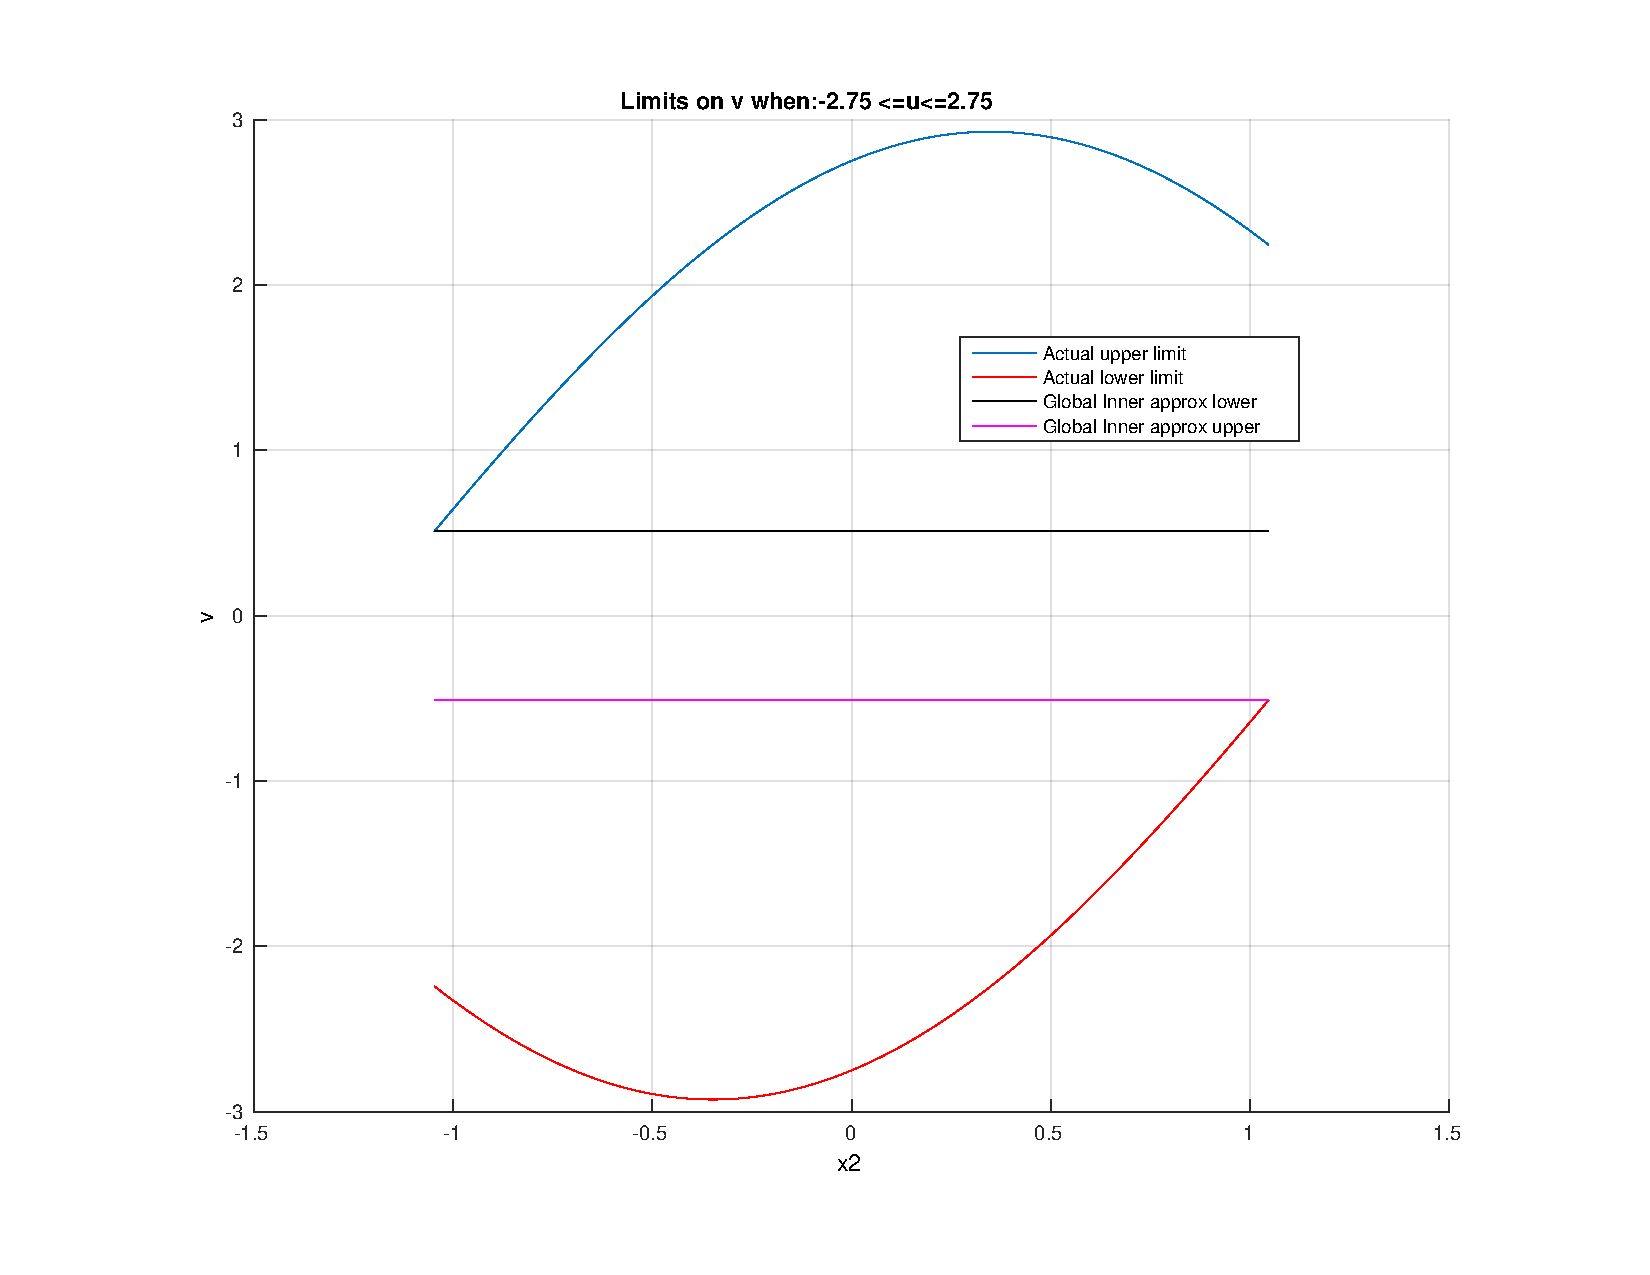
\includegraphics[width=0.46\textwidth]{Figs/v_u_275.pdf}
	\vspace{-10pt}
	\caption{Limits on $v$ (global inner and actual) when $-2.75\leq u \leq 2.75$.}
	\label{fig:v_u_275}%same freq diff assignment}
\end{figure} 

Figs. \ref{fig:v_u_275},\ref{fig:v_u_175} shows the boundaries of the inner approximation and the above actual limits on  the given $X$ and two different $U$. Note, since among the states, $v$ is only a function of $x_2$, we can plot these limits as a function of just $x_2$. Note how quickly the inner approximation shrinks as the bounds on $u$ change from $|u|\leq2.75$ to $|u|\leq1.75$. Also worth noting is that the actual bounds on $v$ form a convex set as function of the state $x$ since the upper limit is concave and the lower limit is convex on the domain $x\in X$.

\begin{figure}[tb]
	\centering
	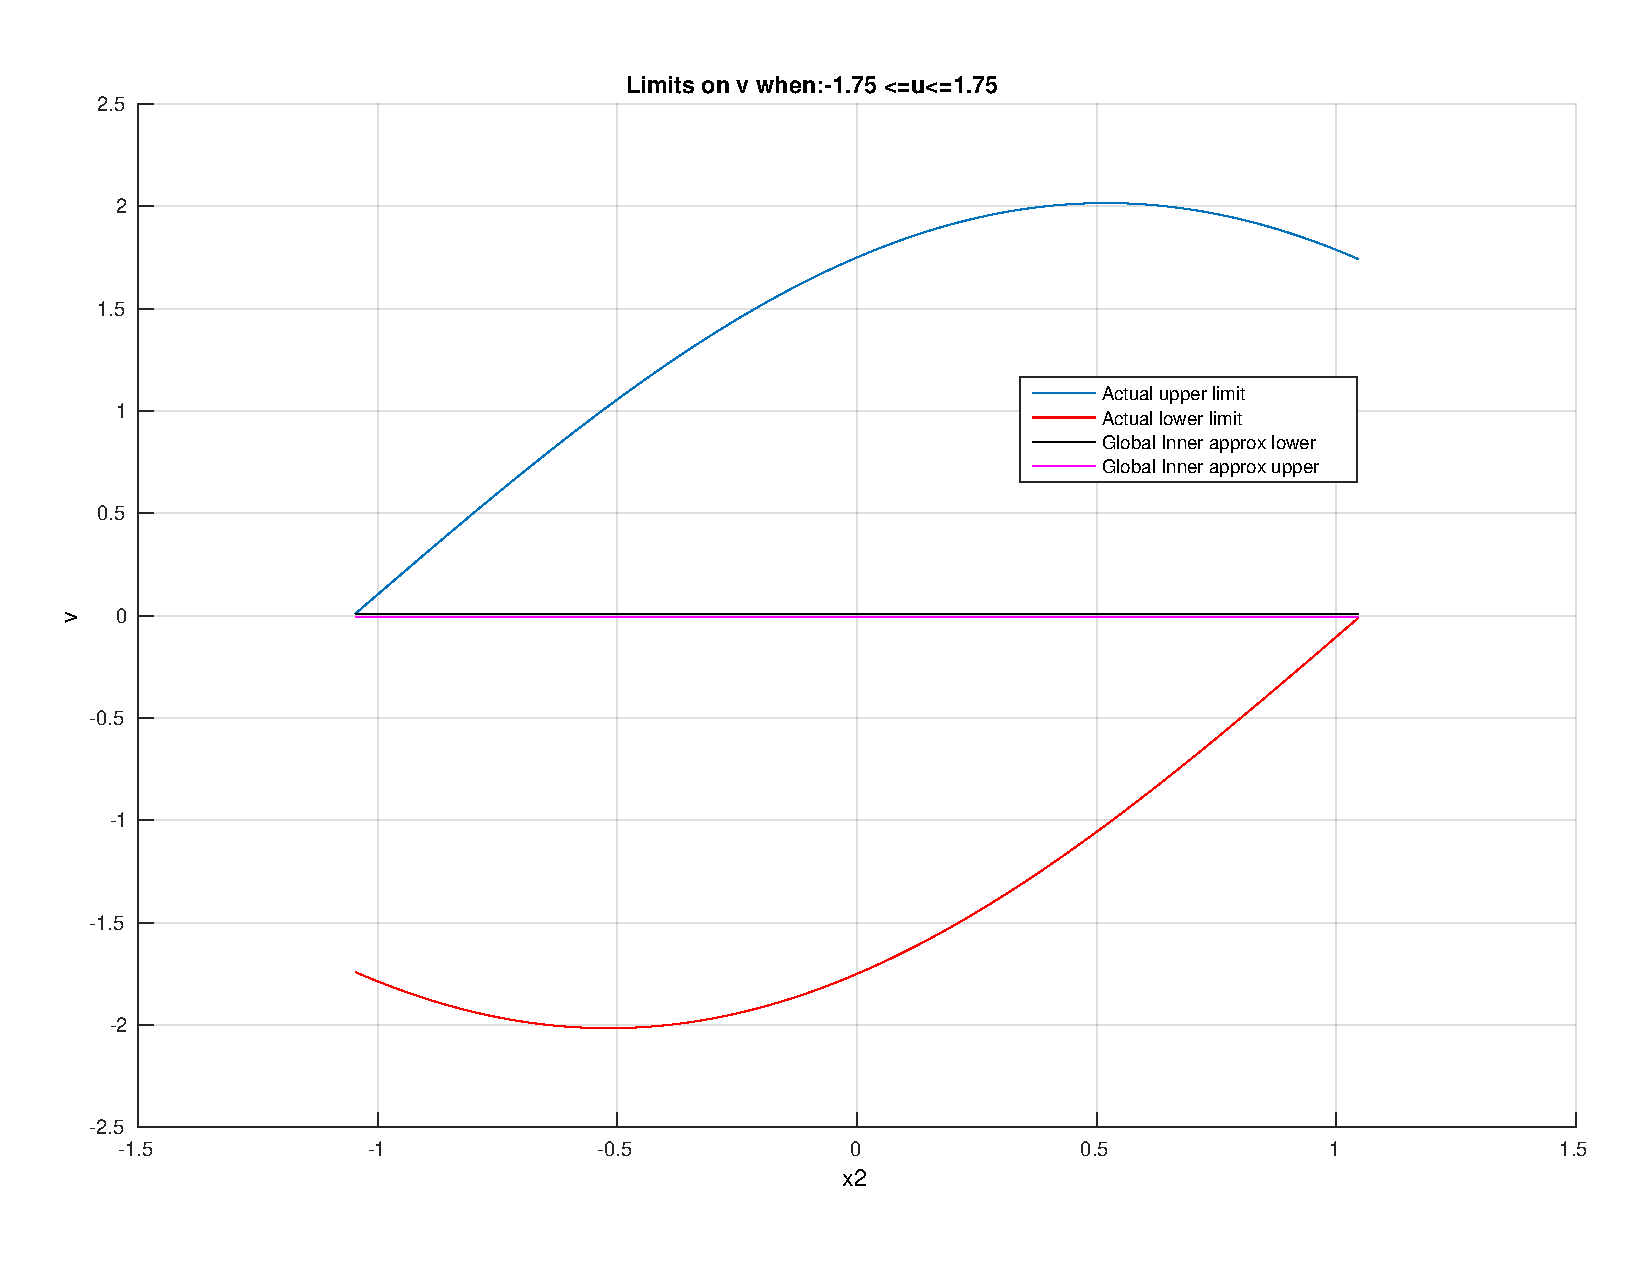
\includegraphics[width=0.46\textwidth]{Figs/v_u_175.pdf}
	\vspace{-10pt}
	\caption{Limits on $v$ (global inner and actual) when $-1.75\leq u \leq 1.75$.}
	\label{fig:v_u_175}%same freq diff assignment}
\end{figure} 


\end{document}

